\documentclass[usenames,dvipsnames,tikz]{standalone}
%\usepackage{xcolor}
%\definecolor{tLightGreen1}{HTML}{B7F385} %tikz color
%\definecolor{tLightOrange1}{HTML}{FFCD4F} %tikz color
%\colorlet{tLightGreen}{LimeGreen!70!OliveGreen!45!White}
%\colorlet{tLightOrange}{Dandelion!65!White}
\definecolor{tLightPink}{HTML}{FFD4EB} %tikz color
\definecolor{tLightBlue}{HTML}{CEF0FF} %tikz color
\colorlet{tRed}{Red}
%\usepackage{tikz}
%\usepackage{standalone}
\begin{document}
	
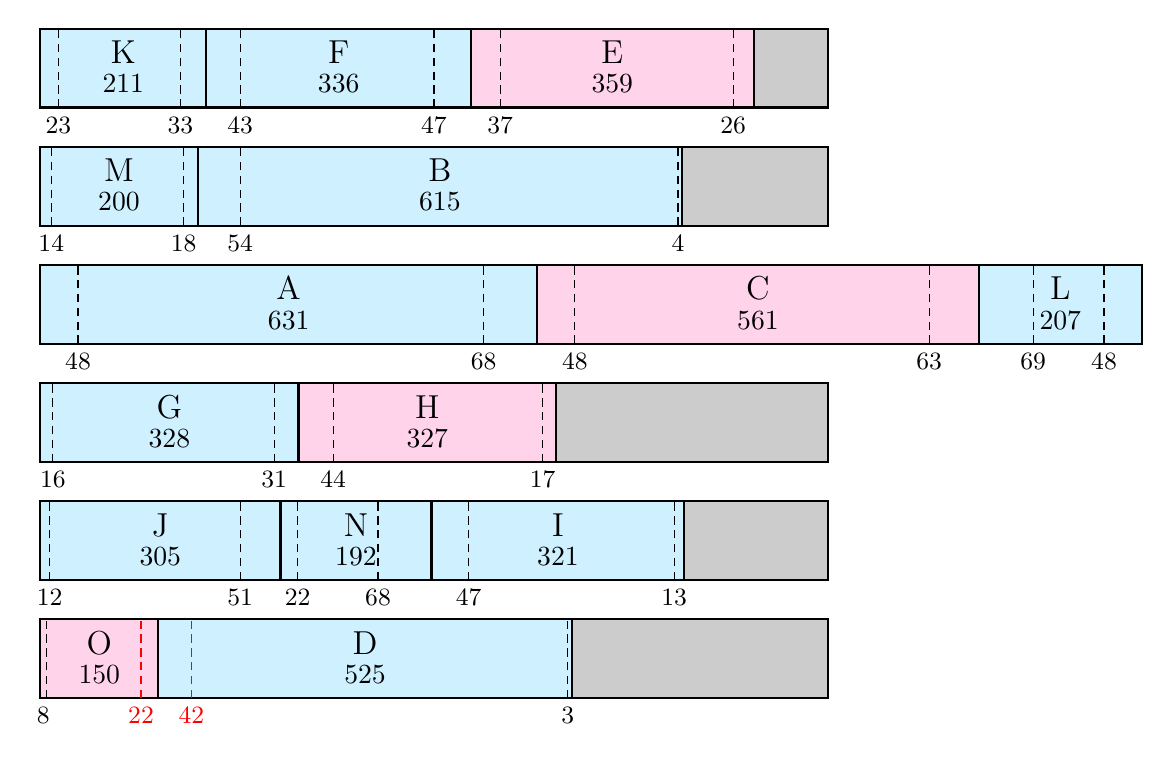
\begin{tikzpicture}
%\draw [help lines] (-1,-2) grid (13,11);

% K, F, E, 211, 336, 359 (23-33, 43-47, 37-26) E FROM OTHER PARENT
\path [fill=tLightBlue] (0,7.5) rectangle (5.47,8.5);
\path [fill=tLightPink] (5.47,7.5) rectangle (9.06,8.5);
\draw [thick] (0,7.5) rectangle (10, 8.5);
\draw [thick] (2.11,7.5) -- (2.11, 8.5);
\draw [thick] (5.47,7.5) -- (5.47, 8.5); % E FROM OTHER PARENT
\draw [thick] (9.06,7.5) -- (9.06, 8.5);
\filldraw[fill=black!20!white, draw=black, thick] (9.06,7.5) rectangle (10,8.5);
\draw [densely dashed] (0.23,7.5) -- (0.23,8.5);
\draw [densely dashed] (1.78,7.5) -- (1.78,8.5);
\draw [densely dashed] (2.54,7.5) -- (2.54,8.5);
\draw [densely dashed] (5.00,7.5) -- (5.00,8.5);
\draw [densely dashed] (5.84,7.5) -- (5.84,8.5);
\draw [densely dashed] (8.8,7.5) -- (8.8,8.5);
\node at (1.055,7.8) {$211$};
\node at (3.79,7.8) {$336$};
\node at (7.265,7.8) {$359$};
\node at (1.055,8.2) {\large K};
\node at (3.79,8.2) {\large F};
\node at (7.265,8.2) {\large E}; 
\node [below] at (0.23,7.5) {\small$23$};
\node [below] at (1.78,7.5) {\small$33$};
\node [below] at (2.54,7.5) {\small$43$};
\node [below] at (5.00,7.5) {\small$47$};
\node [below] at (5.84,7.5) {\small$37$};
\node [below] at (8.8,7.5) {\small$26$};

% M, B, 200, 615 (14-18, 54-4)
\path [fill=tLightBlue] (0,6) rectangle (8.15,7);
\draw [thick] (0,6) rectangle (10, 7);
\draw [thick] (2,6) -- (2,7);
\filldraw[fill=black!20!white, draw=black, thick] (8.15,6) rectangle (10,7);
\draw [densely dashed] (0.14,6) -- (0.14,7);
\draw [densely dashed] (1.82,6) -- (1.82,7);
\draw [densely dashed] (2.54,6) -- (2.54,7);
\draw [densely dashed] (8.1,6) -- (8.1,7);
\node at (1,6.3) {$200$};
\node at (5.075,6.3) {$615$};
\node at (1,6.7) {\large M};
\node at (5.075,6.7) {\large B};
\node [below] at (0.14,6) {\small$14$};
\node [below] at (1.82,6) {\small$18$};
\node [below] at (2.54,6) {\small$54$};
\node [below] at (8.1,6) {\small$4$};


% A, C, L, 631, 561, 207 (48-68, 48-63, 69-48) (OVERFULL) C FROM OTHER PARENT
\path [fill=tLightBlue] (0,4.5) rectangle (6.31,5.5);
\path [fill=tLightPink] (6.31,4.5) rectangle (11.92,5.5);
\path [fill=tLightBlue] (11.92,4.5) rectangle (13.99,5.5);
\draw [thick] (0,4.5) rectangle (13.99, 5.5);
\draw [thick] (6.31,4.5) -- (6.31,5.5);
\draw [thick] (11.92,4.5) -- (11.92,5.5); % C FROM OTHER PARENT
\draw [thick] (13.99,4.5) -- (13.99,5.5);
%\filldraw[fill=black!20!white, draw=black, thick] (9.88,4.5) rectangle (10,5.5);
\draw [densely dashed] (0.48,4.5) -- (0.48,5.5);
\draw [densely dashed] (5.63,4.5) -- (5.63,5.5);
\draw [densely dashed] (6.79,4.5) -- (6.79,5.5);
\draw [densely dashed] (11.29,4.5) -- (11.29,5.5);
\draw [densely dashed] (12.61,4.5) -- (12.61,5.5);
\draw [densely dashed] (13.51,4.5) -- (13.51,5.5);
\node at (3.155,4.8) {$631$};
\node at (9.115,4.8) {$561$};
\node at (12.955,4.8) {$207$};
\node at (3.155,5.2) {\large A};
\node at (9.115,5.2) {\large C};
\node at (12.955,5.2) {\large L};
\node [below] at (0.48,4.5) {\small$48$};
\node [below] at (5.63,4.5) {\small$68$};
\node [below] at (6.79,4.5) {\small$48$};
\node [below] at (11.29,4.5) {\small$63$};
\node [below] at (12.61,4.5) {\small$69$};
\node [below] at (13.51,4.5) {\small$48$};

% G, H, 328, 327 (16-31, 44-17) H FROM OTHER PARENT
\path [fill=tLightBlue] (0,3) rectangle (3.28,4);
\path [fill=tLightPink] (3.28,3) rectangle (6.55,4);
\draw [thick] (0,3) rectangle (10,4);
\draw [thick] (3.28,3) -- (3.28,4);
\draw [thick] (6.55,3) -- (6.55,4); % H FROM OTHER PARENT
\filldraw[fill=black!20!white, draw=black, thick] (6.55,3) rectangle (10,4);
\draw [densely dashed] (0.16,3) -- (0.16,4);
\draw [densely dashed] (2.97,3) -- (2.97,4);
\draw [densely dashed] (3.72,3) -- (3.72,4);
\draw [densely dashed] (6.38,3) -- (6.38,4);
\node at (1.64,3.3) {$328$};
\node at (4.915,3.3) {$327$};
\node at (1.64,3.7) {\large G};
\node at (4.915,3.7) {\large H};
\node [below] at (0.16,3) {\small$16$};
\node [below] at (2.97,3) {\small$31$};
\node [below] at (3.72,3) {\small$44$};
\node [below] at (6.38,3) {\small$17$};


% J, N, I, 305, 192, 321 (12-51, 22-68, 47-13)
\path [fill=tLightBlue] (0,1.5) rectangle (8.18,2.5);
\draw [thick] (0,1.5) rectangle (10, 2.5);
\draw [thick] (3.05,1.5) -- (3.05,2.5);
\draw [thick] (4.97,1.5) -- (4.97,2.5);
\filldraw[fill=black!20!white, draw=black, thick] (8.18,1.5) rectangle (10,2.5);
\draw [densely dashed] (0.12,1.5) -- (0.12,2.5);
\draw [densely dashed] (2.54,1.5) -- (2.54,2.5);
\draw [densely dashed] (3.27,1.5) -- (3.27,2.5);
\draw [densely dashed] (4.29,1.5) -- (4.29,2.5);
\draw [densely dashed] (5.44,1.5) -- (5.44,2.5);
\draw [densely dashed] (8.05,1.5) -- (8.05,2.5);
\node at (1.525,1.8) {$305$};
\node at (4.01,1.8) {$192$};
\node at (6.575,1.8) {$321$};
\node at (1.525,2.2) {\large J};
\node at (4.01,2.2) {\large N};
\node at (6.575,2.2) {\large I};
\node [below] at (0.12,1.5) {\small$12$};
\node [below] at (2.54,1.5) {\small$51$};
\node [below] at (3.27,1.5) {\small$22$};
\node [below] at (4.29,1.5) {\small$68$};
\node [below] at (5.44,1.5) {\small$47$};
\node [below] at (8.05,1.5) {\small$13$};


% O, D 150, 525 (8-22 X 42-3) (VSC NOT MET) O FROM OTHER PARENT
\path [fill=tLightPink] (0,0) rectangle (1.5,1);
\path [fill=tLightBlue] (1.5,0) rectangle (6.75,1);
\draw [thick] (0,0) rectangle (10,1); 
\draw [thick] (1.5,0) -- (1.5,1);% O FROM OTHER PARENT
\draw [thick] (6.75,0) -- (6.75,1);
\filldraw[fill=black!20!white, draw=black, thick] (6.75,0) rectangle (10,1);
\draw [densely dashed] (0.08,0) -- (0.08,1);
\draw [densely dashed, tRed] (1.28,0) -- (1.28,1);
\draw [densely dashed, tRed] (1.92,0) -- (1.92,1);
\draw [densely dashed] (6.70,0) -- (6.70,1);
\node at (0.75,0.3) {$150$};
\node at (4.125,0.3) {$525$};
\node at (0.75,0.7) {\large O};
\node at (4.125,0.7) {\large D};
\node [below] at (0.04,0) {\small$8$};
\node [below] at (1.28,0) {\textcolor{tRed}{\small$22$}};
\node [below] at (1.92,0) {\textcolor{tRed}{\small$42$}};
\node [below] at (6.70,0) {\small$3$};

%\node at (5, -1.5) {\huge{$\mathcal{S}_2$}};

\end{tikzpicture}
	
\end{document}